\chapter*{Outline ET 250-3D turntable control}
In this appendix the control of an Outline ET 250-3D turntable will be described. The turntable can be controlled in three ways, first the turntable can be controlled by \gls{ttl} commands through a jack connector. Secondly the turntable can be controlled by specified \gls{dll} command through Ethernet. All commands is included in the software packed folder. Thirdly the turntable can be controlled by \gls{udp} command through Ethernet. For controlling the turntable by MATLAB, the two Ethernet based control method is the easiest to do because MATLAB support Ethernet access. The \gls{dll} method require a complicated scripted which might only work on Windows operation system. The \gls{udp} can run at all operation system which support IPv4 Ethernet connection and is a short simple script, where the script open a \gls{udp} channel as a file, and e.g.  the script shall only edit the file in the right position to move the turntable. The chosen control method is \gls{udp} because it is simple and works at all modern computer operation systems.

\section*{Materials and setup}
The following materials are used:
\begin{itemize}
\item Ethernet cable
\item Outline ET 250-3D (Turntable)
\item MATLAB (PC - software)
\end{itemize}

%\begin{figure}[htbp!]
%\centering
%\def\svgwidth{\columnwidth}
%\chapter{Test of the Guitar's Frequency Area}\label{app:frequency_area}
A test was made to get an overview of the frequency area in which the tones from the guitar lie.

\section*{Materials and Setup}
To measure the frequency area on a guitar, the following materials are used:
\begin{itemize}
\item Digilent Analog Discovery 2 (Oscilloscope)
\item Fender Squier Classic Vibe Telecaster (Guitar)
\item Digilent Waveforms 2015 (PC - software)
\end{itemize}

\begin{figure}[htbp!]
\centering
\def\svgwidth{\columnwidth}
\chapter{Test of the Guitar's Frequency Area}\label{app:frequency_area}
A test was made to get an overview of the frequency area in which the tones from the guitar lie.

\section*{Materials and Setup}
To measure the frequency area on a guitar, the following materials are used:
\begin{itemize}
\item Digilent Analog Discovery 2 (Oscilloscope)
\item Fender Squier Classic Vibe Telecaster (Guitar)
\item Digilent Waveforms 2015 (PC - software)
\end{itemize}

\begin{figure}[htbp!]
\centering
\def\svgwidth{\columnwidth}
\chapter{Test of the Guitar's Frequency Area}\label{app:frequency_area}
A test was made to get an overview of the frequency area in which the tones from the guitar lie.

\section*{Materials and Setup}
To measure the frequency area on a guitar, the following materials are used:
\begin{itemize}
\item Digilent Analog Discovery 2 (Oscilloscope)
\item Fender Squier Classic Vibe Telecaster (Guitar)
\item Digilent Waveforms 2015 (PC - software)
\end{itemize}

\begin{figure}[htbp!]
\centering
\def\svgwidth{\columnwidth}
\input{figures/appendix/guitar_frequency_test.pdf_tex}
\caption{Setup for measuring frequency area on a guitar.}
		\label{fig:appendix:guitar_freq}
\end{figure}

\section*{Test Procedure}
To measure the frequency area on a guitar, the following steps are followed:
\begin{enumerate}
\item The materials are set up as in \autoref{fig:appendix:guitar_freq}.
\item Digilent Waveforms 2015 is set as a spectrum analyser. 
\item The guitar is set to use the neck pickup, the volume and tone control are turned all the way up to their maximum.
\item The highest and the lowest tone on the guitar are played, measured by the oscilloscope and analysed in Digilent Waveforms 2015.
\item The guitar is set to use the bridge pickup and step 4 is repeated. 
\item The data is plotted in MATLAB.
\end{enumerate}

\section*{Results}

\begin{figure}[htbp!]
	\centering
		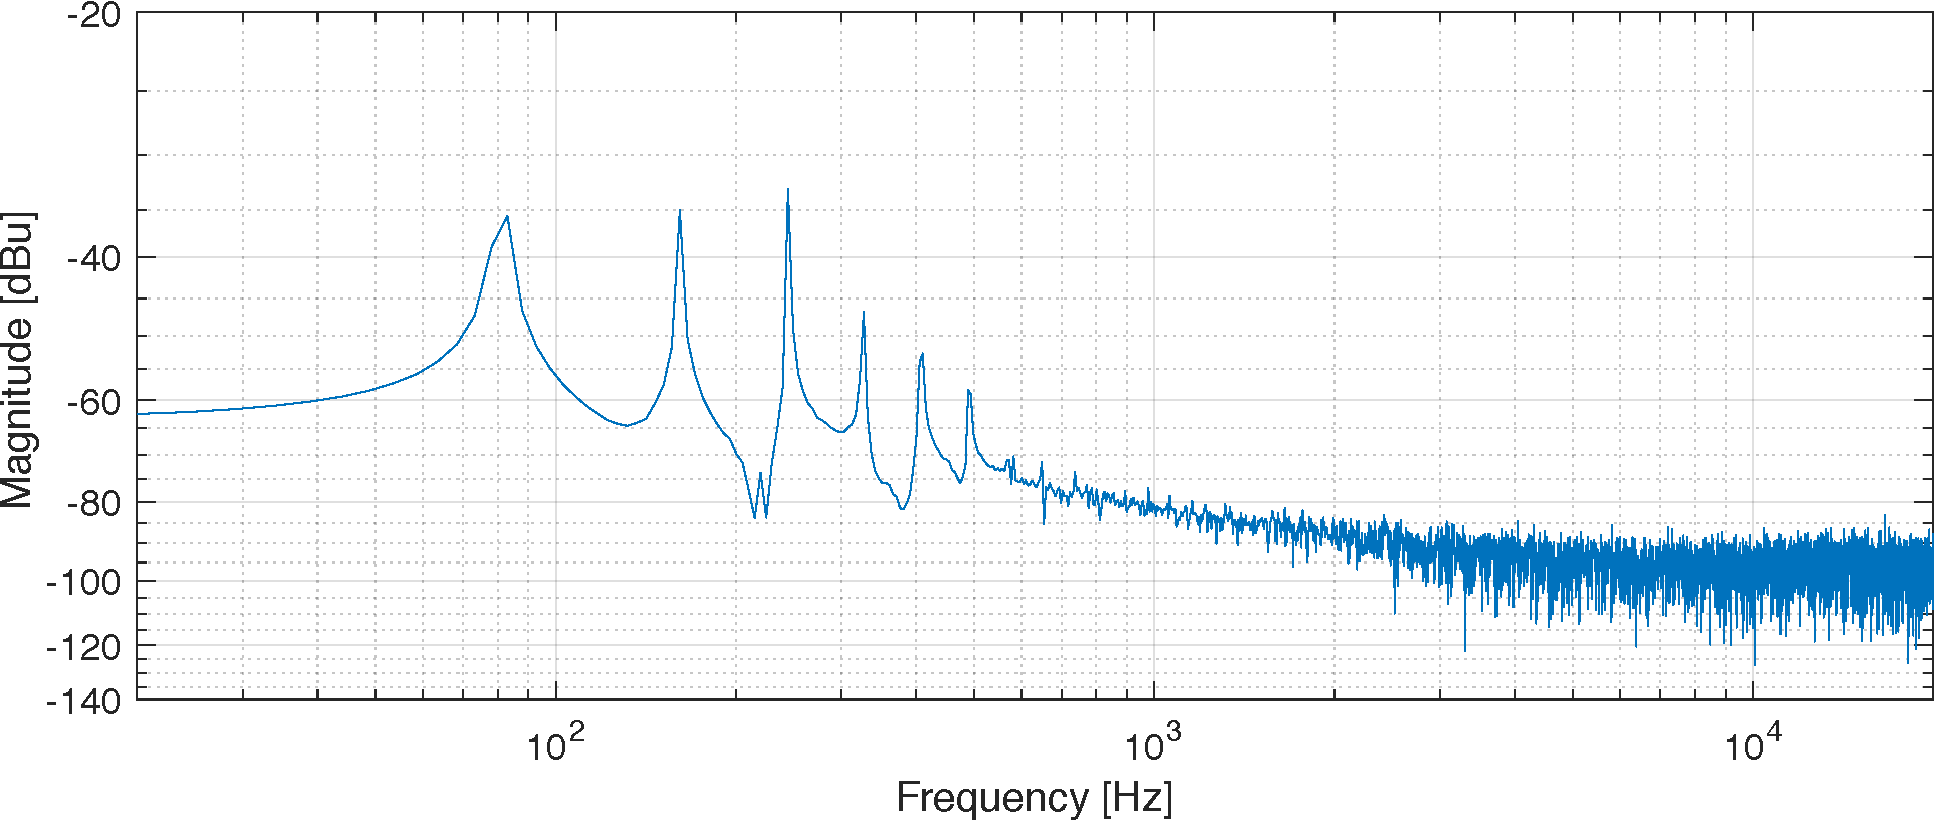
\includegraphics[width=1\textwidth]{guitar_low_E_neck.pdf}
		\caption{Measurement of the low E note on the neck pickup.}
		\label{fig:appendix:low_E_neck}
\end{figure}

On \autoref{fig:appendix:low_E_neck} it is seen that the lowest significant frequency is around \SI{80}{\hertz} and the highest significant frequency is around \SI{500}{\hertz}, when playing the low E note on the guitar, using the neck pickup.

\newpage
\begin{figure}[htbp!]
	\centering
		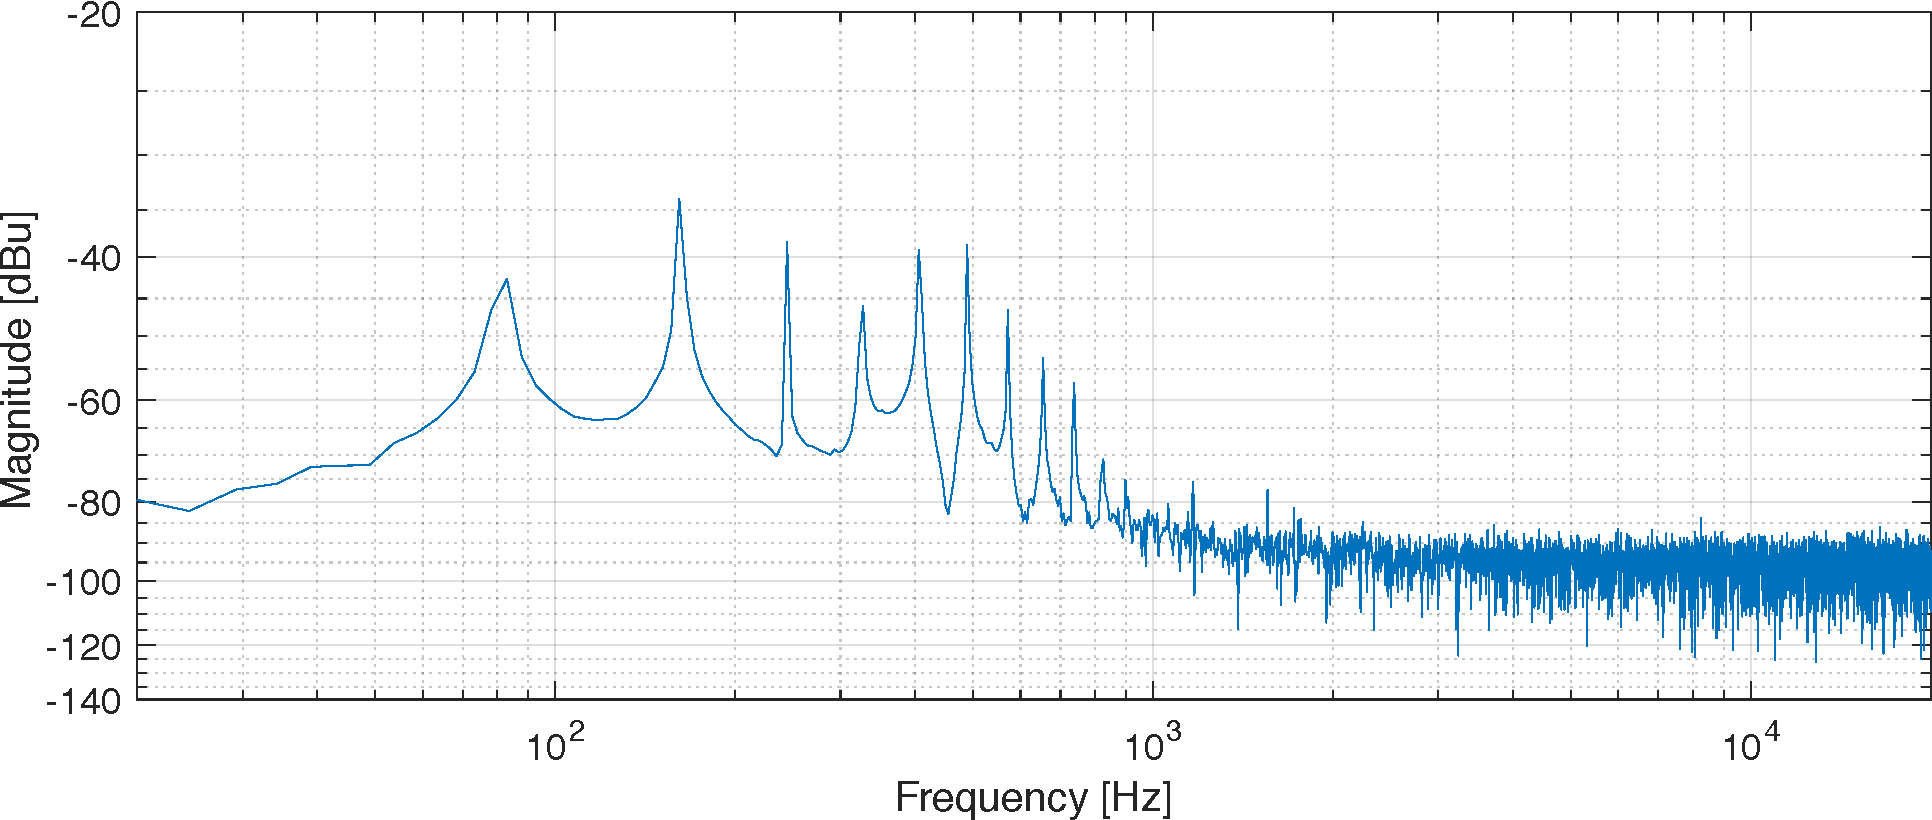
\includegraphics[width=1\textwidth]{guitar_low_E_bridge.pdf}
		\caption{Measurement of the low E note on the bridge pickup.}
		\label{fig:appendix:low_E_bridge}
\end{figure}

On  \autoref{fig:appendix:low_E_bridge} it is seen that the lowest significant frequency is around \SI{80}{\hertz} and the highest significant frequency is around \SI{730}{\hertz}, when playing the low E note on the guitar, using the bridge pickup.

\begin{figure}[htbp!]
	\centering
		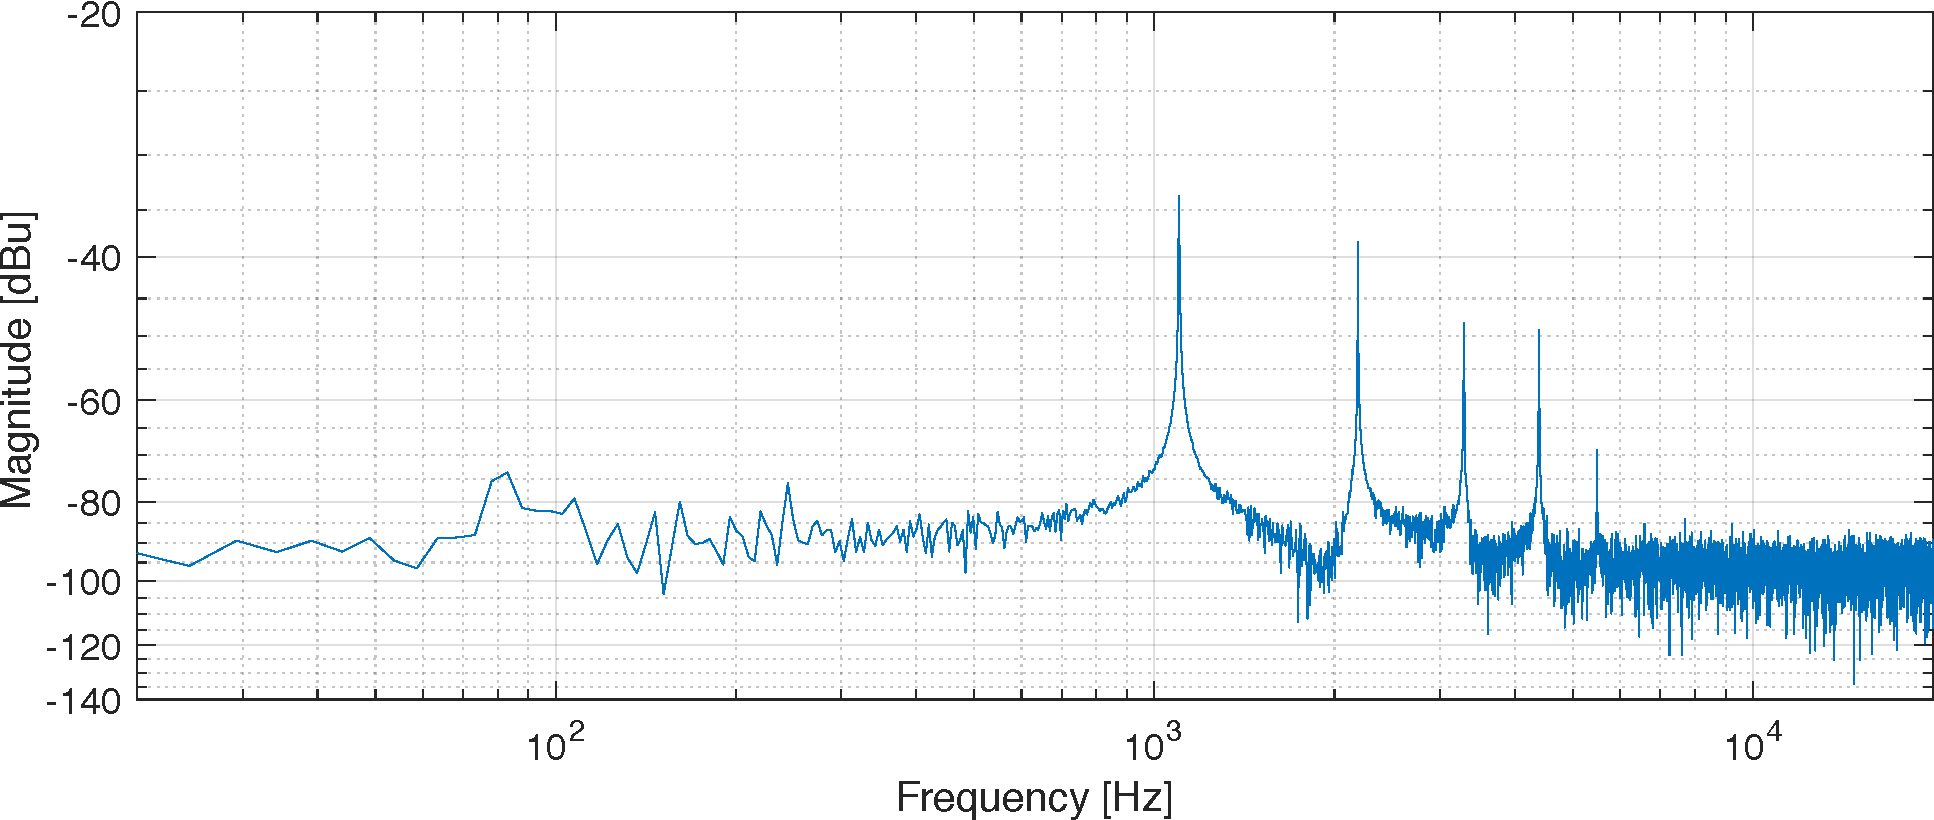
\includegraphics[width=1\textwidth]{guitar_high_Cis_neck.pdf}
		\caption{Measurement of the high C\# note on the neck pickup.}
		\label{fig:appendix:high_Cis_neck}
\end{figure}

On  \autoref{fig:appendix:high_Cis_neck} it is seen that the lowest significant frequency is around \SI{1100}{\hertz} and the highest significant frequency is around \SI{4400}{\hertz}, when playing the high C\# note on the guitar, using the neck pickup.

\newpage
\begin{figure}[htbp!]
	\centering
		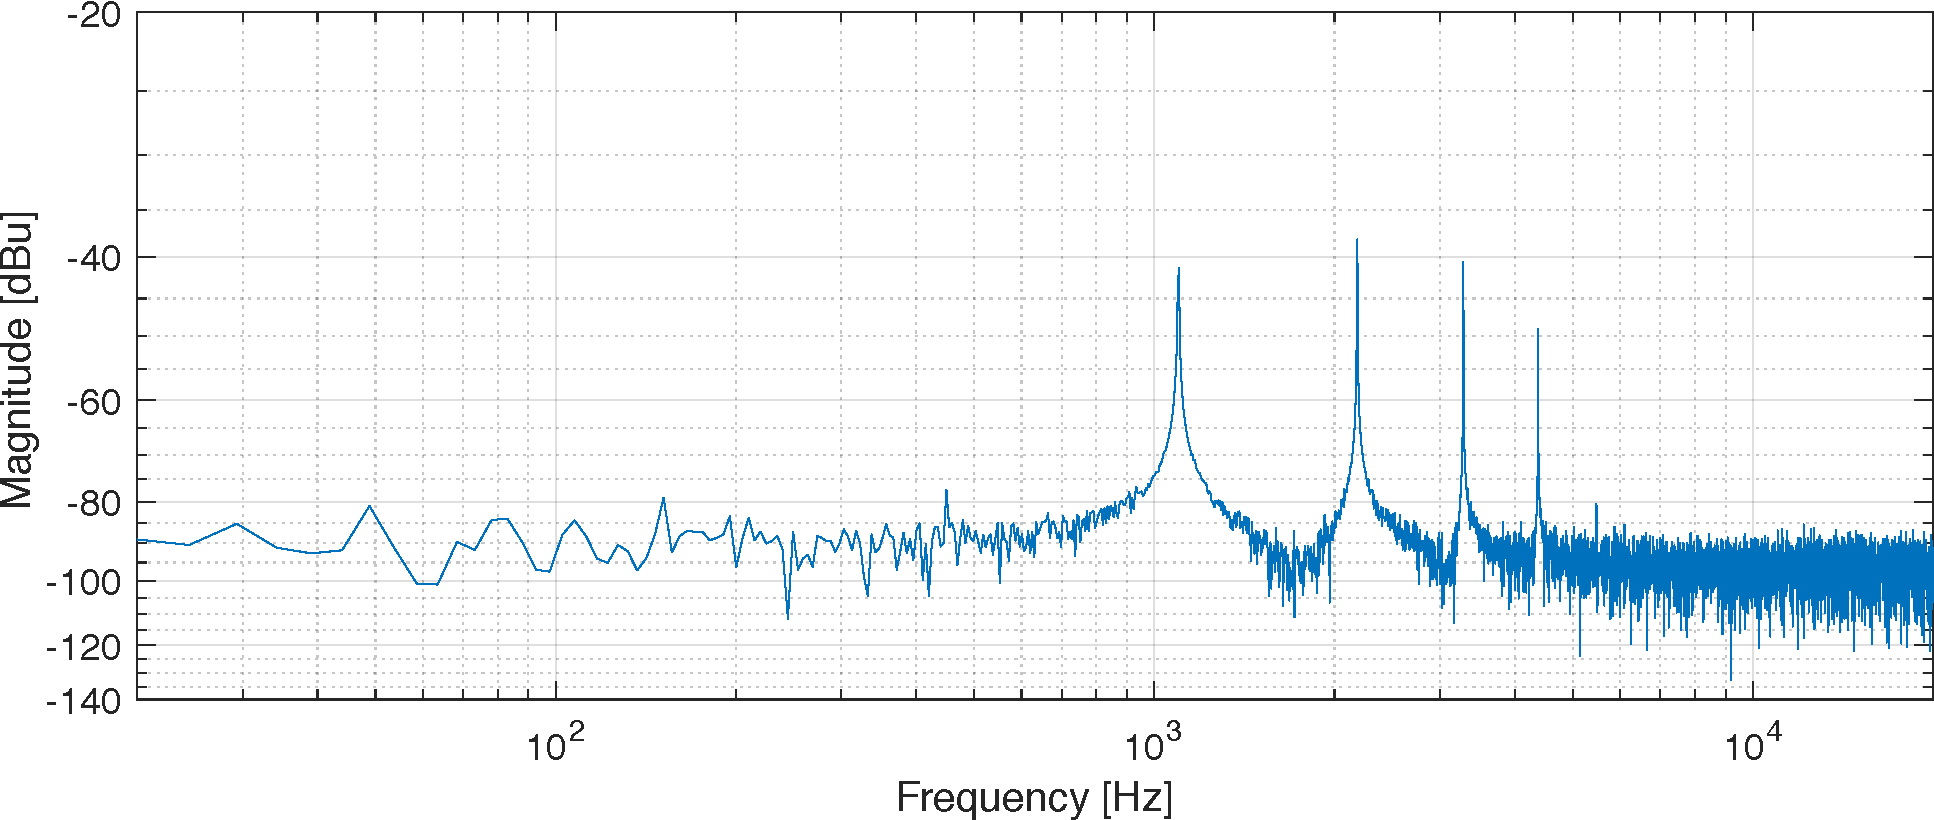
\includegraphics[width=1\textwidth]{guitar_high_Cis_bridge.pdf}
		\caption{Measurement of the high C\# note on the bridge pickup.}
		\label{fig:appendix:high_Cis_bridge}
\end{figure}

On  \autoref{fig:appendix:high_Cis_bridge} it is seen that the lowest significant frequency is around \SI{1100}{\hertz} and the highest significant frequency is around \SI{4400}{\hertz}, when playing the high C\# note on the guitar, using the bridge pickup. 

\begin{figure}[htbp!]
	\centering
		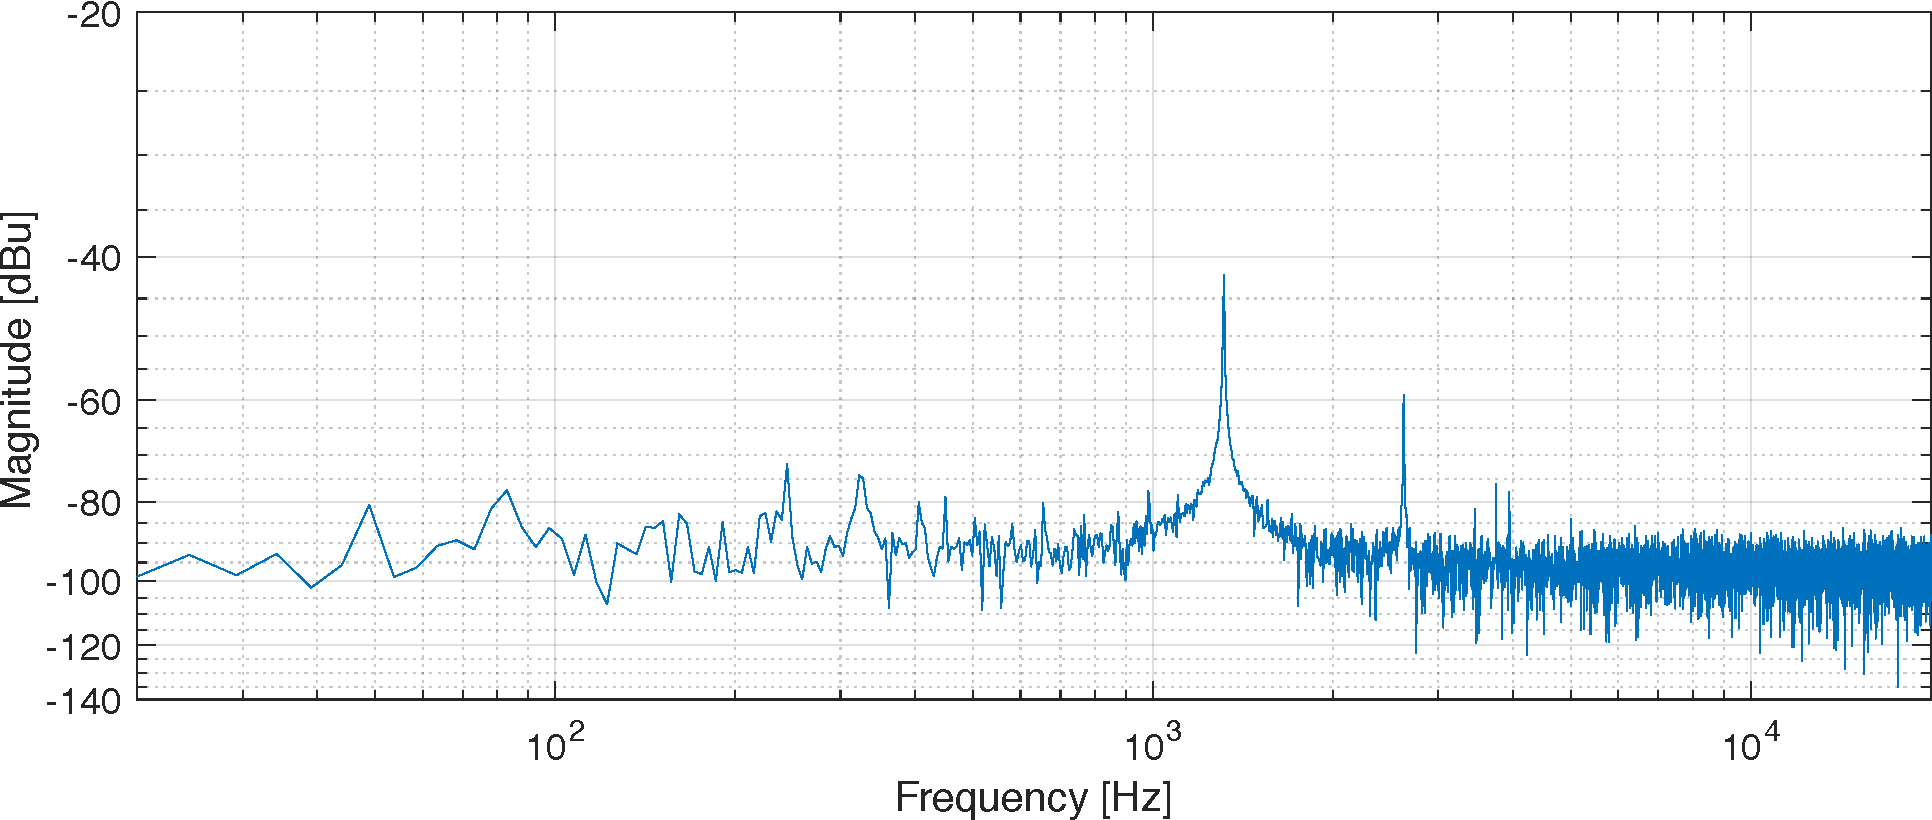
\includegraphics[width=1\textwidth]{guitar_high_E_flasholet_bridge.pdf}
		\caption{Measurement of the high E note, played as flasholet, on the bridge pickup.}
		\label{fig:appendix:high_E_bridge_flasholet}
\end{figure}

On  \autoref{fig:appendix:high_E_bridge_flasholet} it is seen that the lowest significant frequency is around \SI{1300}{\hertz} and the highest significant frequency is around \SI{2600}{\hertz}, when playing the high E note on the guitar as flasholet, using the bridge pickup. 

\caption{Setup for measuring frequency area on a guitar.}
		\label{fig:appendix:guitar_freq}
\end{figure}

\section*{Test Procedure}
To measure the frequency area on a guitar, the following steps are followed:
\begin{enumerate}
\item The materials are set up as in \autoref{fig:appendix:guitar_freq}.
\item Digilent Waveforms 2015 is set as a spectrum analyser. 
\item The guitar is set to use the neck pickup, the volume and tone control are turned all the way up to their maximum.
\item The highest and the lowest tone on the guitar are played, measured by the oscilloscope and analysed in Digilent Waveforms 2015.
\item The guitar is set to use the bridge pickup and step 4 is repeated. 
\item The data is plotted in MATLAB.
\end{enumerate}

\section*{Results}

\begin{figure}[htbp!]
	\centering
		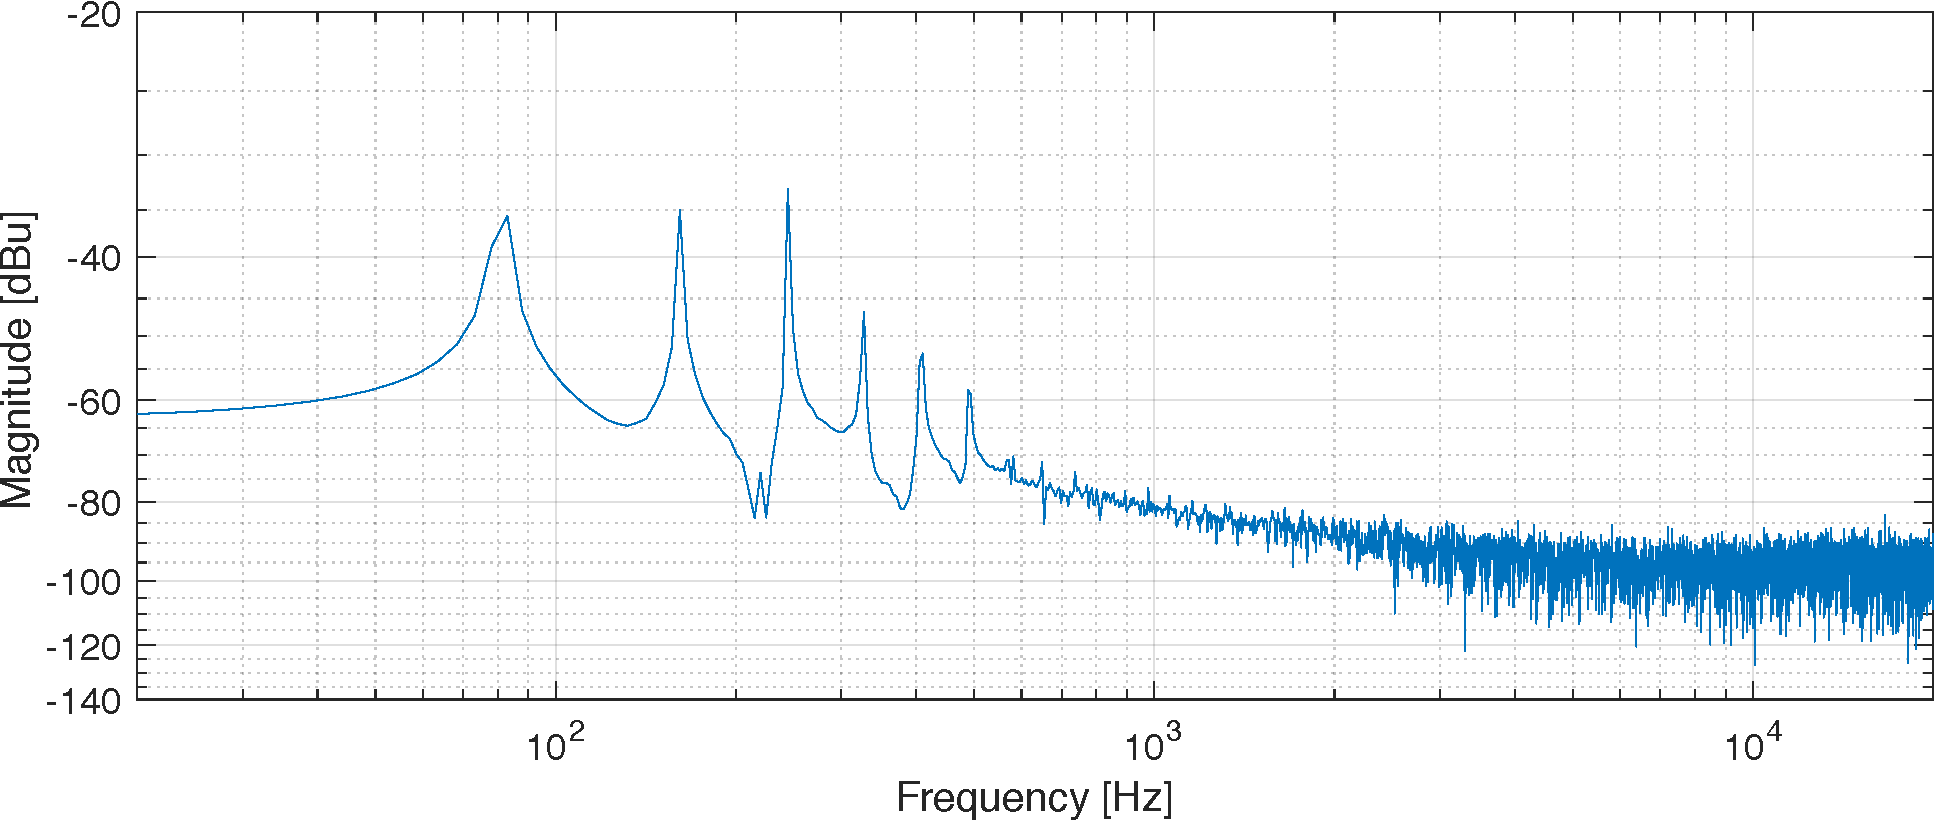
\includegraphics[width=1\textwidth]{guitar_low_E_neck.pdf}
		\caption{Measurement of the low E note on the neck pickup.}
		\label{fig:appendix:low_E_neck}
\end{figure}

On \autoref{fig:appendix:low_E_neck} it is seen that the lowest significant frequency is around \SI{80}{\hertz} and the highest significant frequency is around \SI{500}{\hertz}, when playing the low E note on the guitar, using the neck pickup.

\newpage
\begin{figure}[htbp!]
	\centering
		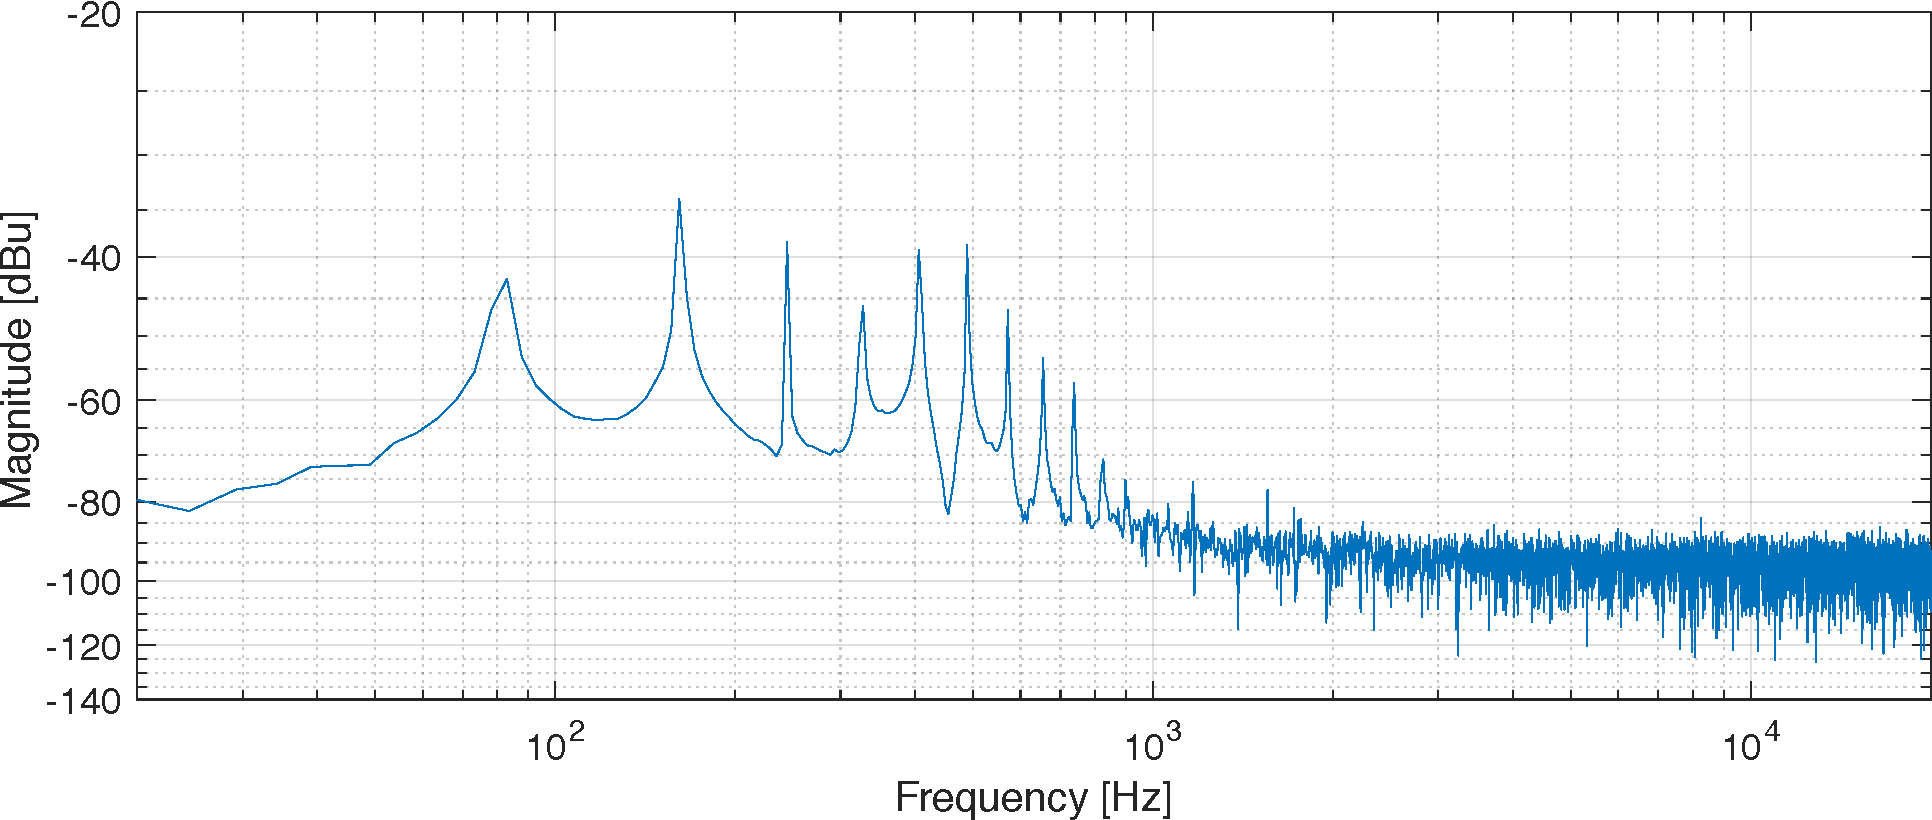
\includegraphics[width=1\textwidth]{guitar_low_E_bridge.pdf}
		\caption{Measurement of the low E note on the bridge pickup.}
		\label{fig:appendix:low_E_bridge}
\end{figure}

On  \autoref{fig:appendix:low_E_bridge} it is seen that the lowest significant frequency is around \SI{80}{\hertz} and the highest significant frequency is around \SI{730}{\hertz}, when playing the low E note on the guitar, using the bridge pickup.

\begin{figure}[htbp!]
	\centering
		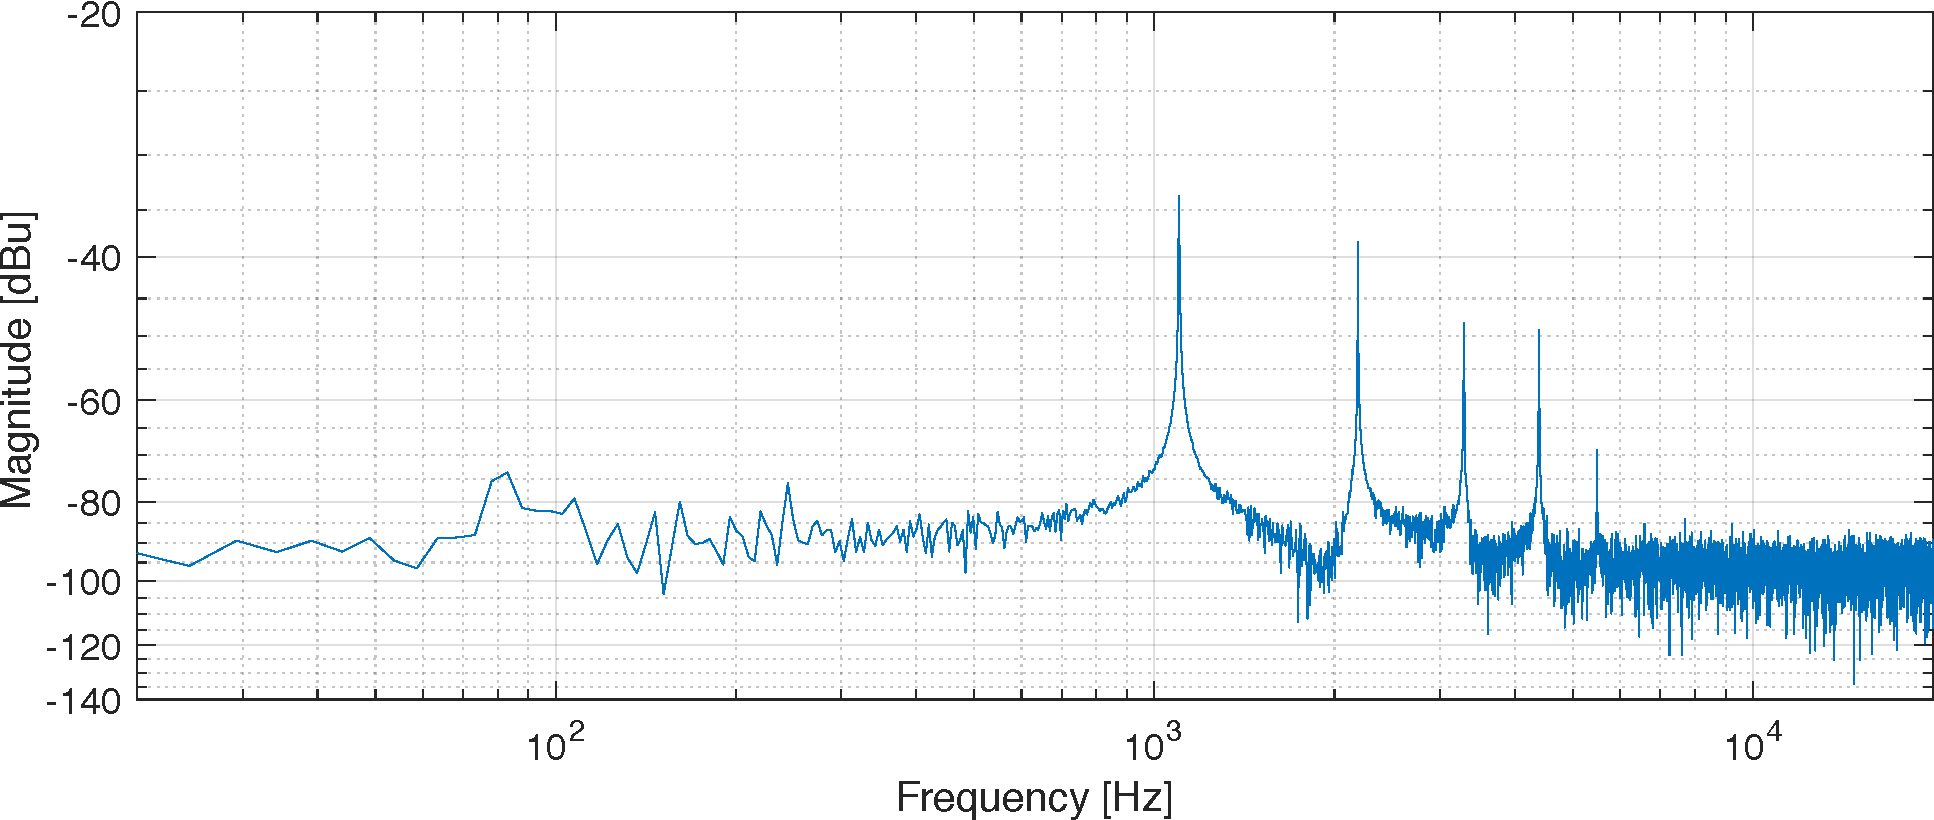
\includegraphics[width=1\textwidth]{guitar_high_Cis_neck.pdf}
		\caption{Measurement of the high C\# note on the neck pickup.}
		\label{fig:appendix:high_Cis_neck}
\end{figure}

On  \autoref{fig:appendix:high_Cis_neck} it is seen that the lowest significant frequency is around \SI{1100}{\hertz} and the highest significant frequency is around \SI{4400}{\hertz}, when playing the high C\# note on the guitar, using the neck pickup.

\newpage
\begin{figure}[htbp!]
	\centering
		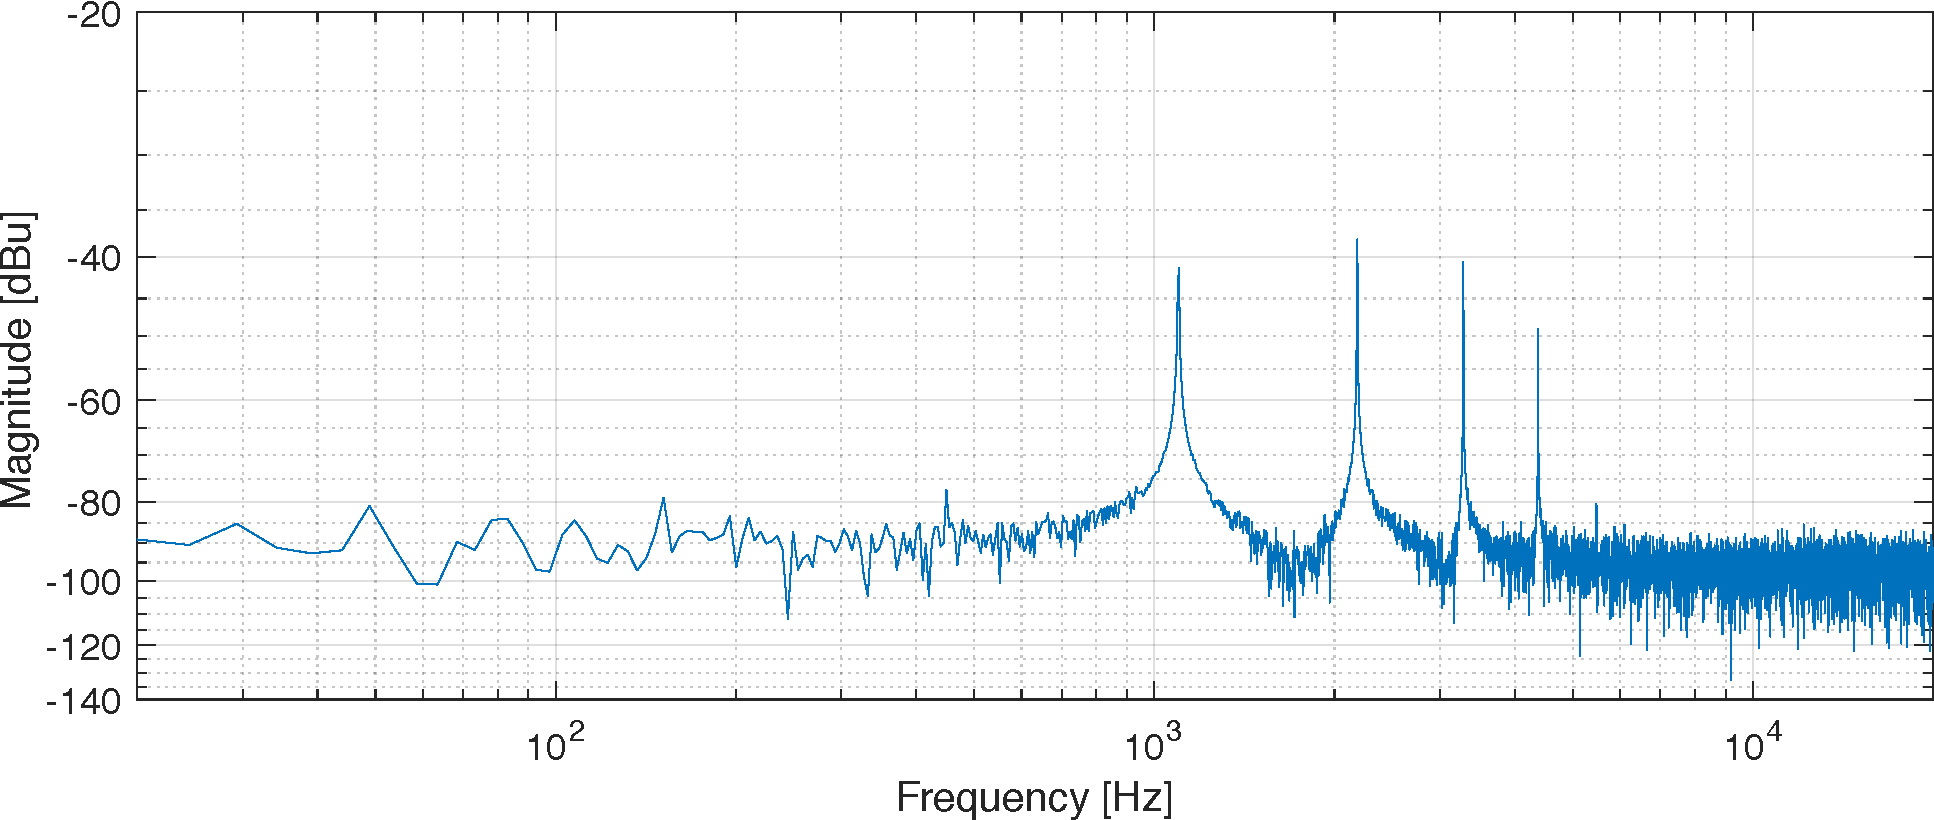
\includegraphics[width=1\textwidth]{guitar_high_Cis_bridge.pdf}
		\caption{Measurement of the high C\# note on the bridge pickup.}
		\label{fig:appendix:high_Cis_bridge}
\end{figure}

On  \autoref{fig:appendix:high_Cis_bridge} it is seen that the lowest significant frequency is around \SI{1100}{\hertz} and the highest significant frequency is around \SI{4400}{\hertz}, when playing the high C\# note on the guitar, using the bridge pickup. 

\begin{figure}[htbp!]
	\centering
		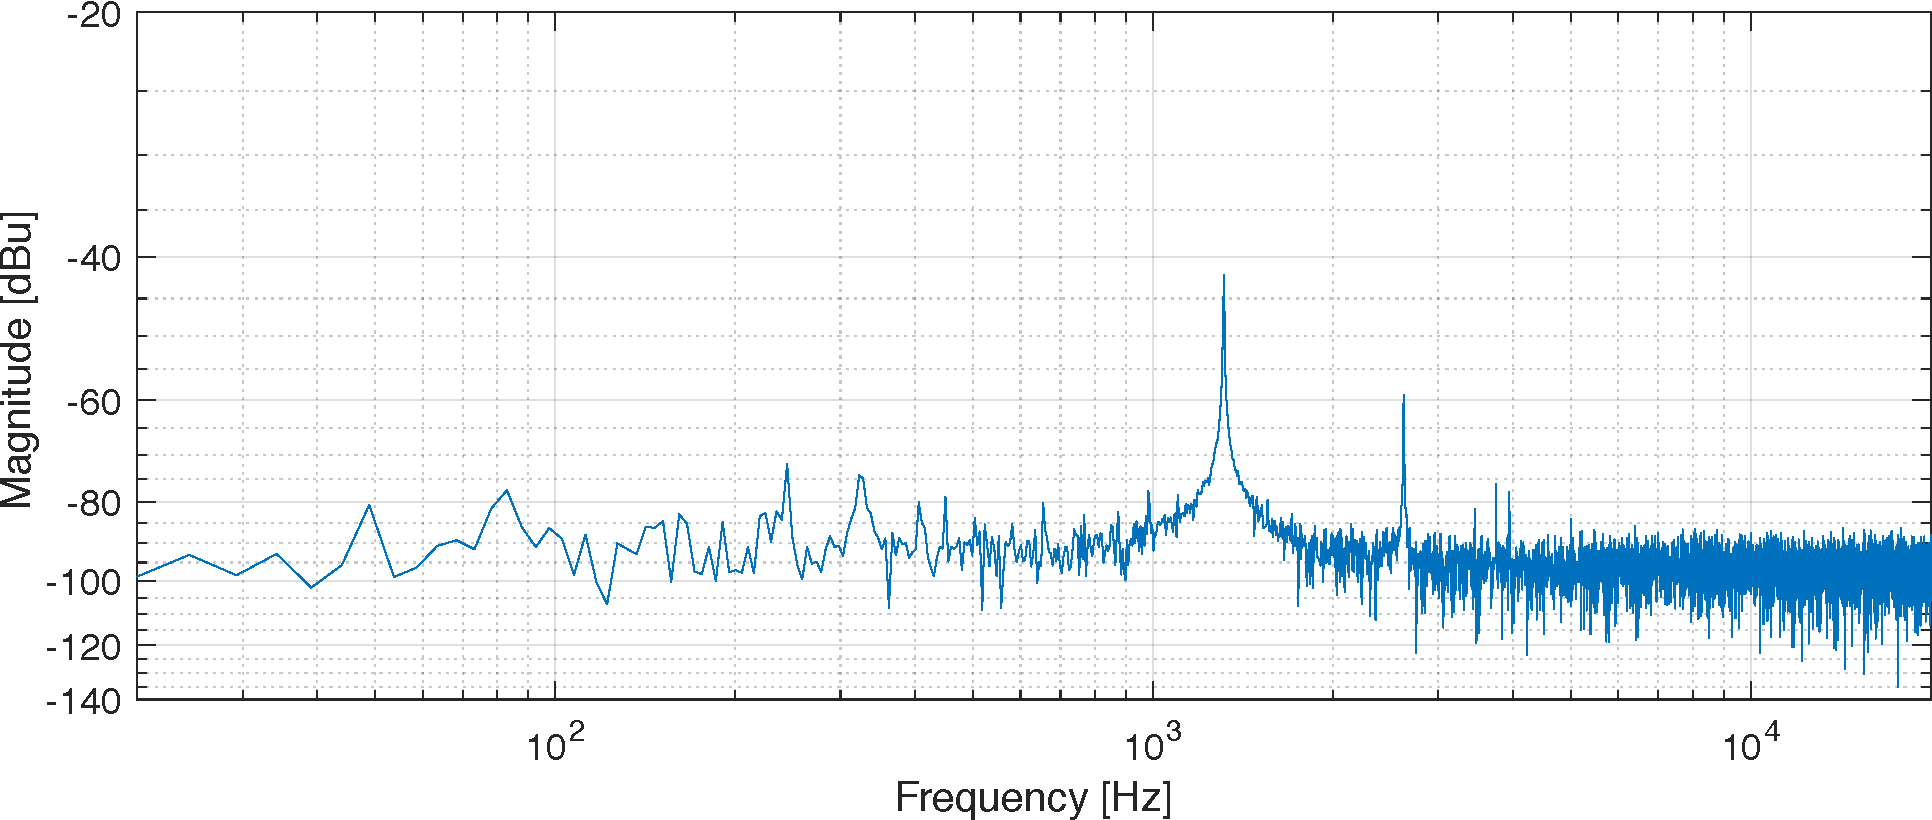
\includegraphics[width=1\textwidth]{guitar_high_E_flasholet_bridge.pdf}
		\caption{Measurement of the high E note, played as flasholet, on the bridge pickup.}
		\label{fig:appendix:high_E_bridge_flasholet}
\end{figure}

On  \autoref{fig:appendix:high_E_bridge_flasholet} it is seen that the lowest significant frequency is around \SI{1300}{\hertz} and the highest significant frequency is around \SI{2600}{\hertz}, when playing the high E note on the guitar as flasholet, using the bridge pickup. 

\caption{Setup for measuring frequency area on a guitar.}
		\label{fig:appendix:guitar_freq}
\end{figure}

\section*{Test Procedure}
To measure the frequency area on a guitar, the following steps are followed:
\begin{enumerate}
\item The materials are set up as in \autoref{fig:appendix:guitar_freq}.
\item Digilent Waveforms 2015 is set as a spectrum analyser. 
\item The guitar is set to use the neck pickup, the volume and tone control are turned all the way up to their maximum.
\item The highest and the lowest tone on the guitar are played, measured by the oscilloscope and analysed in Digilent Waveforms 2015.
\item The guitar is set to use the bridge pickup and step 4 is repeated. 
\item The data is plotted in MATLAB.
\end{enumerate}

\section*{Results}

\begin{figure}[htbp!]
	\centering
		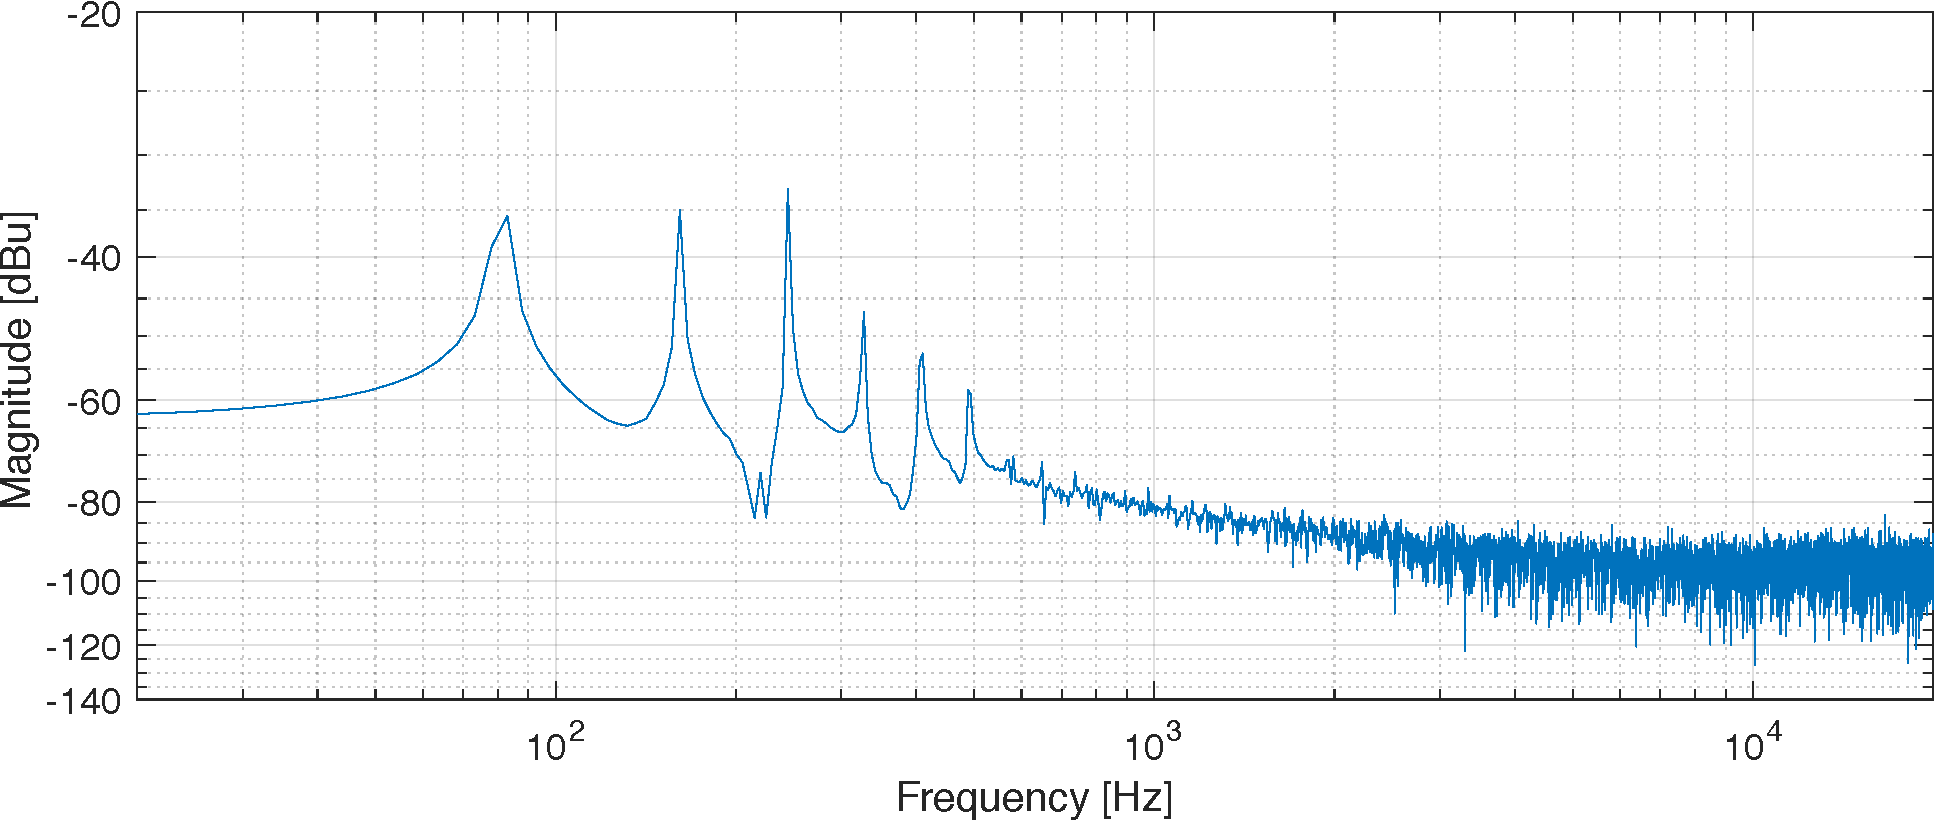
\includegraphics[width=1\textwidth]{guitar_low_E_neck.pdf}
		\caption{Measurement of the low E note on the neck pickup.}
		\label{fig:appendix:low_E_neck}
\end{figure}

On \autoref{fig:appendix:low_E_neck} it is seen that the lowest significant frequency is around \SI{80}{\hertz} and the highest significant frequency is around \SI{500}{\hertz}, when playing the low E note on the guitar, using the neck pickup.

\newpage
\begin{figure}[htbp!]
	\centering
		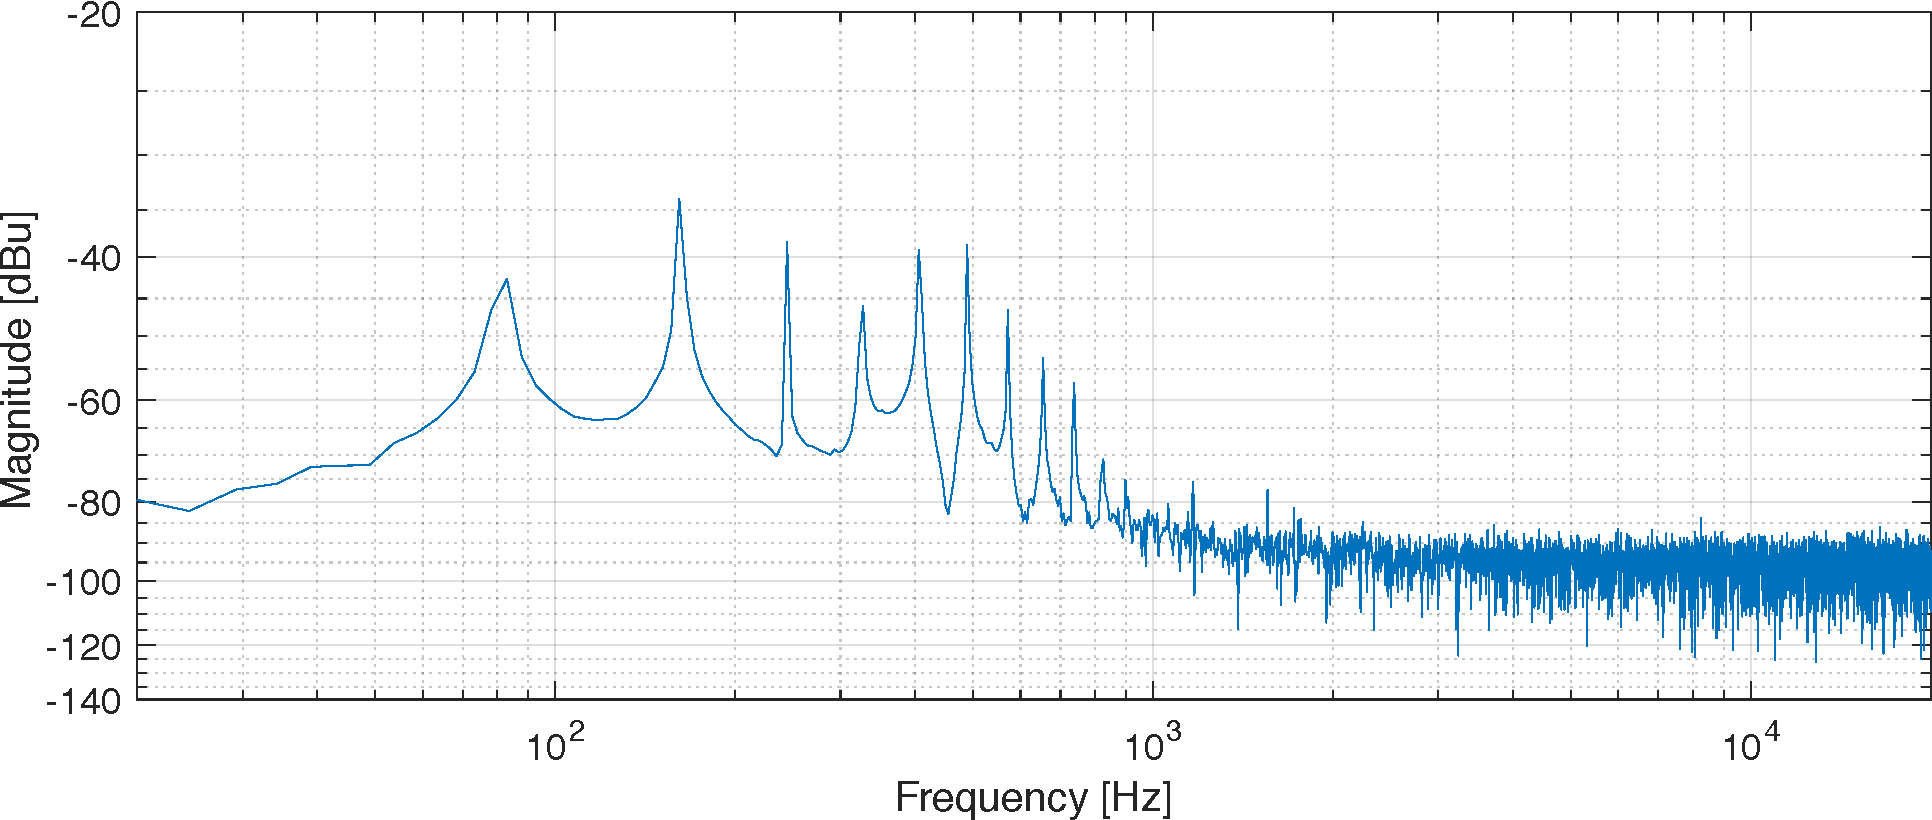
\includegraphics[width=1\textwidth]{guitar_low_E_bridge.pdf}
		\caption{Measurement of the low E note on the bridge pickup.}
		\label{fig:appendix:low_E_bridge}
\end{figure}

On  \autoref{fig:appendix:low_E_bridge} it is seen that the lowest significant frequency is around \SI{80}{\hertz} and the highest significant frequency is around \SI{730}{\hertz}, when playing the low E note on the guitar, using the bridge pickup.

\begin{figure}[htbp!]
	\centering
		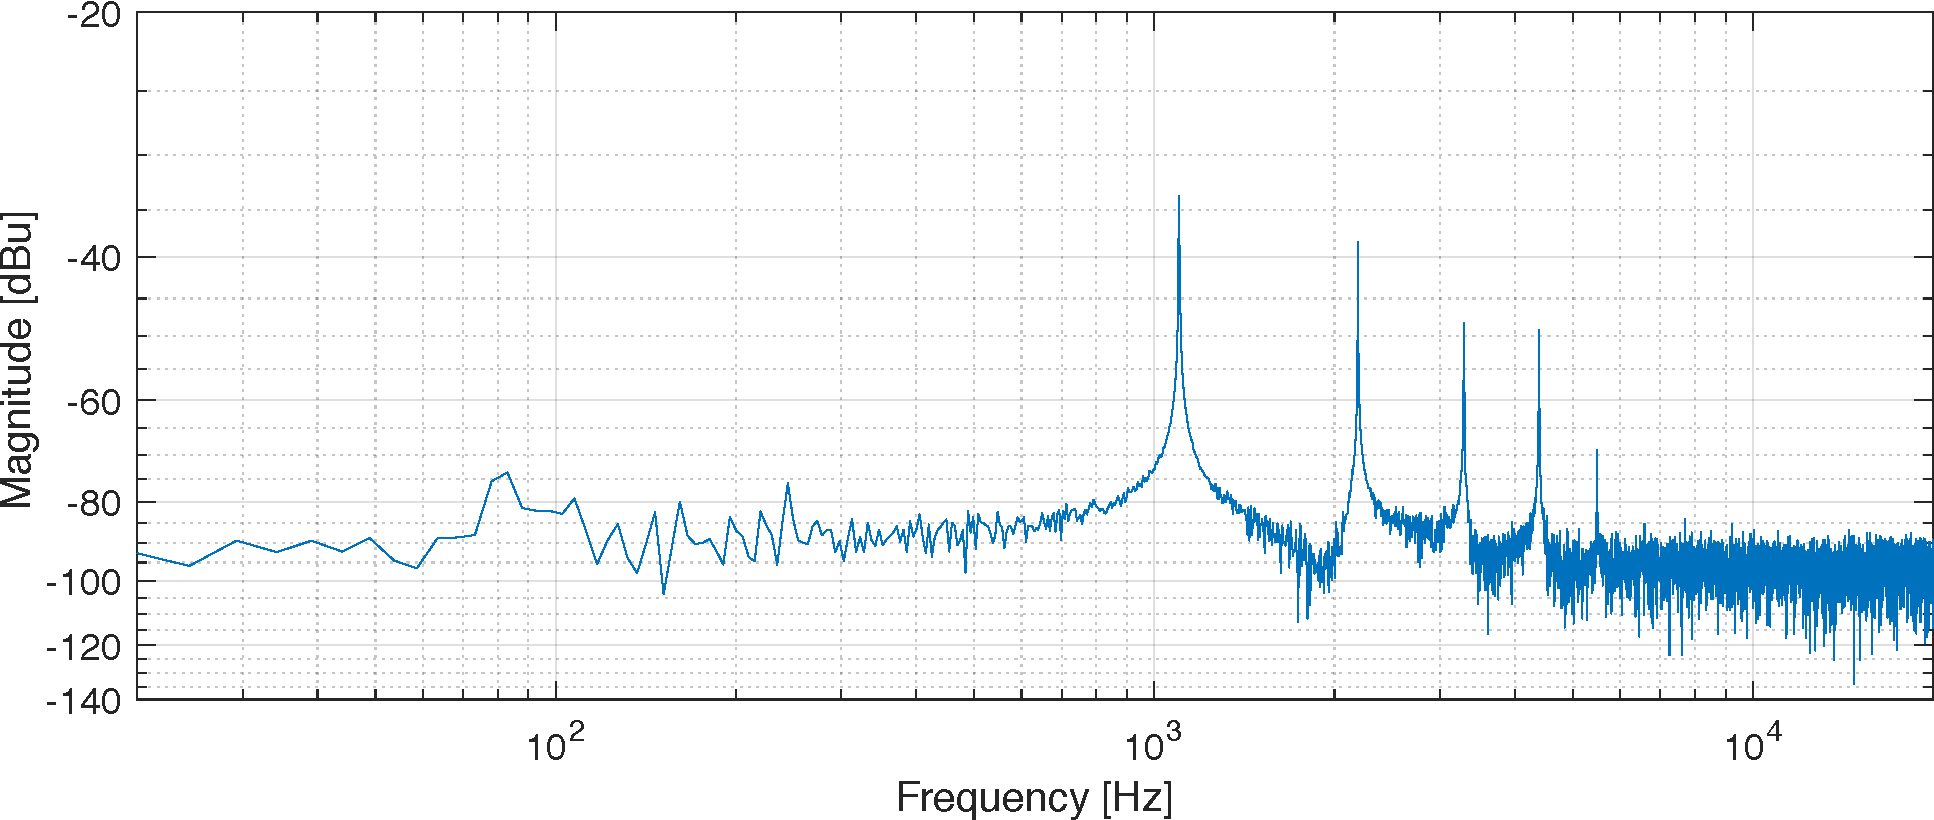
\includegraphics[width=1\textwidth]{guitar_high_Cis_neck.pdf}
		\caption{Measurement of the high C\# note on the neck pickup.}
		\label{fig:appendix:high_Cis_neck}
\end{figure}

On  \autoref{fig:appendix:high_Cis_neck} it is seen that the lowest significant frequency is around \SI{1100}{\hertz} and the highest significant frequency is around \SI{4400}{\hertz}, when playing the high C\# note on the guitar, using the neck pickup.

\newpage
\begin{figure}[htbp!]
	\centering
		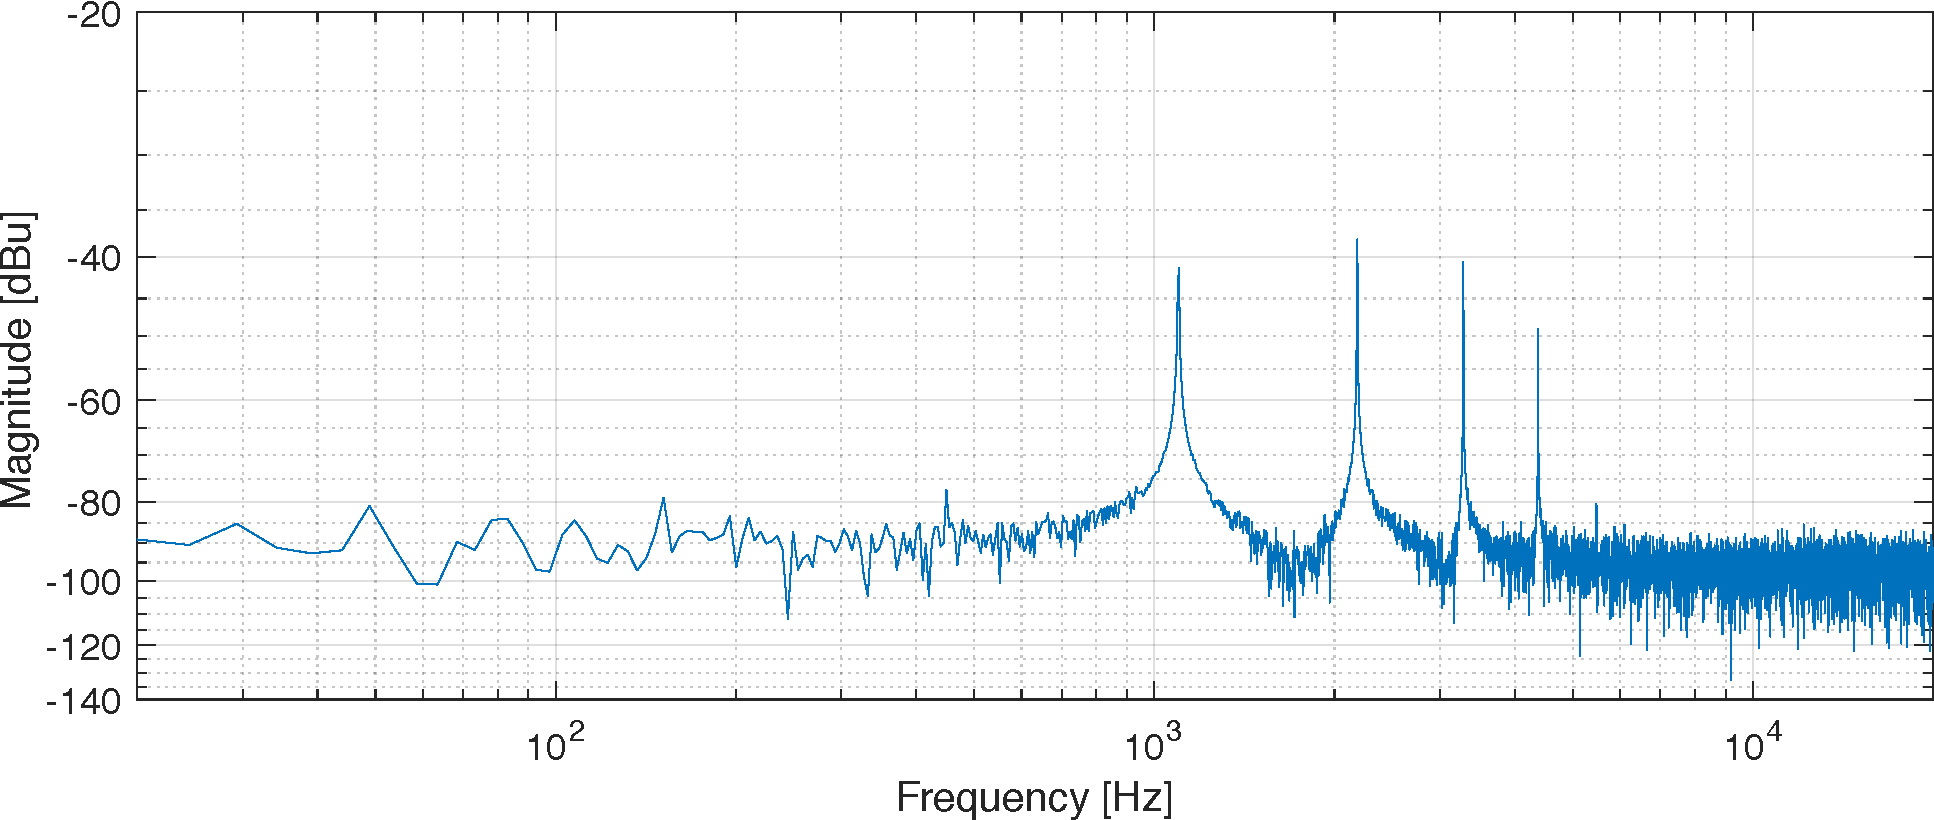
\includegraphics[width=1\textwidth]{guitar_high_Cis_bridge.pdf}
		\caption{Measurement of the high C\# note on the bridge pickup.}
		\label{fig:appendix:high_Cis_bridge}
\end{figure}

On  \autoref{fig:appendix:high_Cis_bridge} it is seen that the lowest significant frequency is around \SI{1100}{\hertz} and the highest significant frequency is around \SI{4400}{\hertz}, when playing the high C\# note on the guitar, using the bridge pickup. 

\begin{figure}[htbp!]
	\centering
		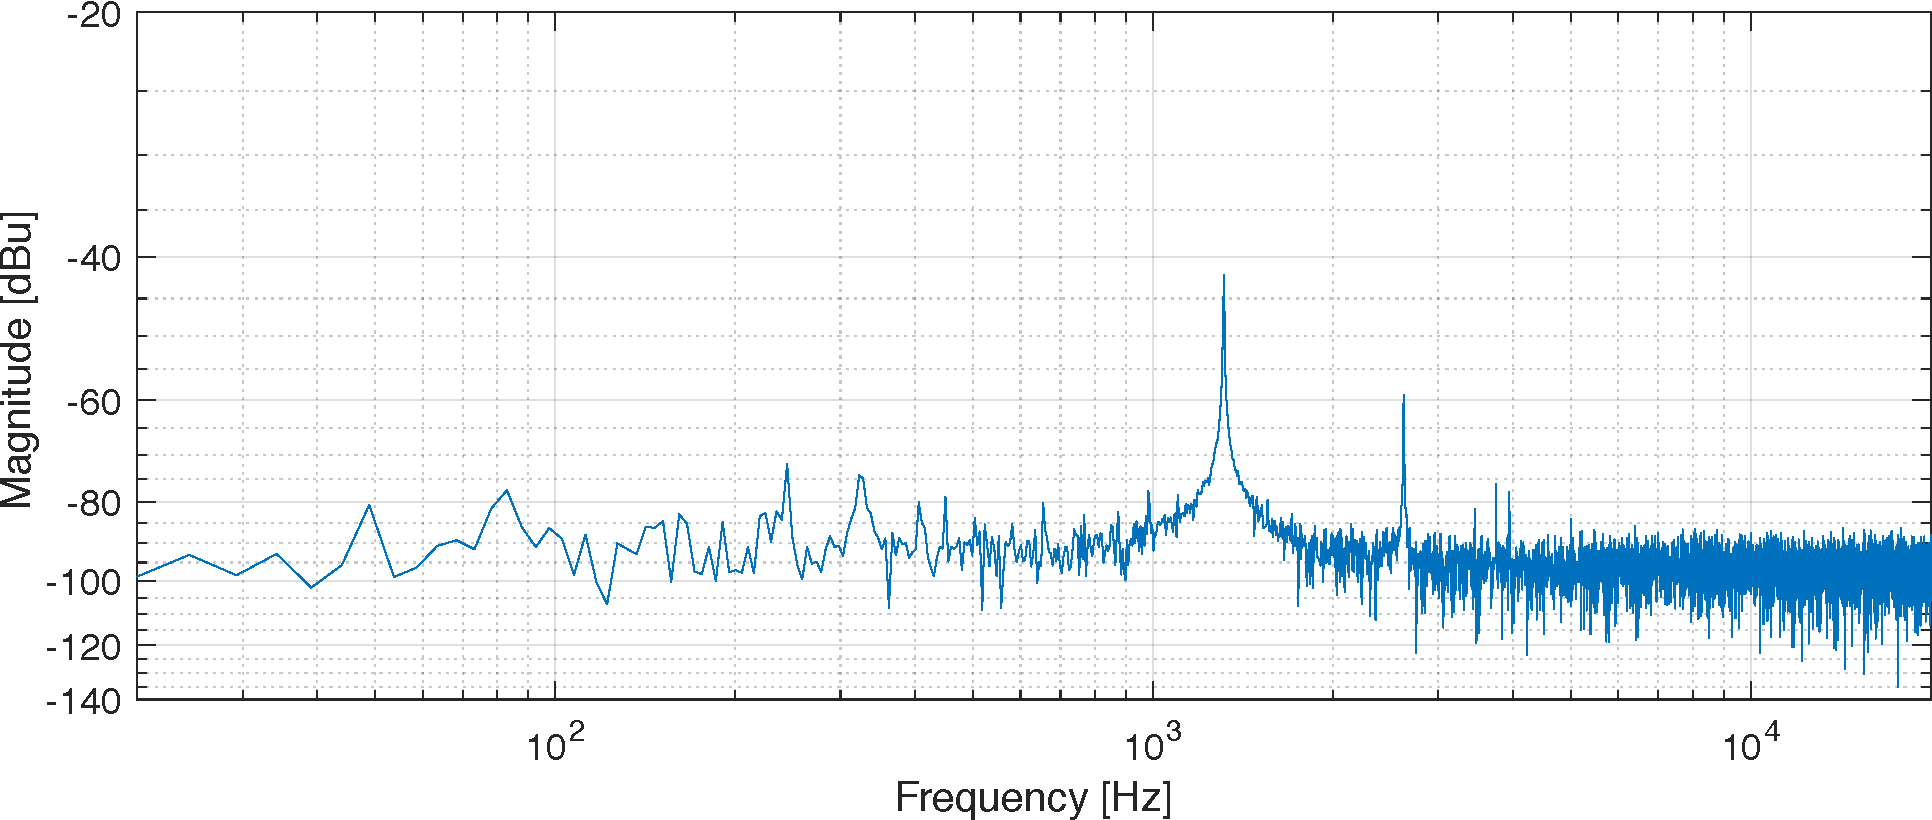
\includegraphics[width=1\textwidth]{guitar_high_E_flasholet_bridge.pdf}
		\caption{Measurement of the high E note, played as flasholet, on the bridge pickup.}
		\label{fig:appendix:high_E_bridge_flasholet}
\end{figure}

On  \autoref{fig:appendix:high_E_bridge_flasholet} it is seen that the lowest significant frequency is around \SI{1300}{\hertz} and the highest significant frequency is around \SI{2600}{\hertz}, when playing the high E note on the guitar as flasholet, using the bridge pickup. 

%\caption{Setup for measuring frequency area on a guitar.}
%		\label{fig:appendix:test}
%\end{figure}

\section*{The \gls{udp} setup of the computer}
To establish connection between the turntable and computer, both have to run at the same SUBNET MASK. The turntable have a factory set for Ethernet connection which is as following:

\begin{table}[H]
\centering
\caption{Turntable network address}
\label{my-label}
\begin{tabular}{lll}
 & \gls{ip} & 192.168.1.34   \\
 & SUBNET MASK  & 255.255.255.0   \\
 & DEFAULT GATEWAY  & 192.168.1.250  \\
 & BROADCAST IP   &  192.168.1.255   
\end{tabular}
\end{table}



\section*{Turntable control command}
The software is made as a function where one can get a position, specify a position and stop the turntable. The function name is:

\includeCode{ET250_3D.m}{matlab}{1}{1}{The turntable control function}{code:ET250_3D}{./code/turntable/}

The function is made as an switch case with input variable "cmd", and an angle input. The following command can be send to the "cmd" of the function:

 \begin{table}[H]
\centering
\caption{Function command}
\label{my-label}
\begin{tabular}{lll}
 & $cmd = 'udp_start'$ & Which start a connection on port 7000 \\
 & $cmd = 'set'$ & Which move the turntable to the specified angle    \\
 & $cmd = 'get'$ & Which get the position of the turntable and store is as the output variable   \\
 & $cmd = 'stop'$  & Which stop the turntable from moving \\
 & $cmd = 'udp_stop'$ & Which stop the connection on port 7000 
\end{tabular}
\end{table}




\section*{The MATLAB function}

\includeCode{ET250_3D.m}{matlab}{1}{55}{The turntable control function}{code:ET250_3D}{./code/turntable/}




